\documentclass[12pt]{article}
\usepackage[swedish]{babel}
\usepackage[T1]{fontenc}{
\usepackage[utf8]{inputenc}
\usepackage{amssymb}
\usepackage{amsmath}
\usepackage{amsfonts}
\usepackage[colorinlistoftodos,prependcaption,textsize=small]{todonotes}
\usepackage{url,graphicx,tabularx,array,geometry,color,float,placeins}
\setlength{\parskip}{1ex} %--skip lines between paragraphs
\setlength{\parindent}{0pt} %--don't indent paragraphs
%\setcounter{secnumdepth}0}
\usepackage{tikz}
\usetikzlibrary{shapes, arrows, 3d, decorations, calc, decorations.markings}

\tikzstyle{block} = [draw, rectangle, thick, minimum height=3em, minimum width=2em, align=center, text width=1.5cm, top color=white, bottom color=white!85!black]
\tikzstyle{input} = [coordinate]
\tikzstyle{output} = [coordinate]
\tikzstyle{tmp} = [coordinate]
\tikzstyle{sum} = [draw, circle, node distance=1cm]
\tikzstyle{wire} = [->,thick]
\tikzstyle{lab} = []
\tikzstyle{laba} = [lab, label distance=0cm]
\tikzstyle{labb} = [lab, label distance=0.5em]
\tikzstyle{split} = [fill,black,circle,inner sep=0.03cm]
\tikzset{cross/.style={cross out, draw=black, minimum size=2*(#1-\pgflinewidth), inner sep=0pt, outer sep=0pt},
%default radius will be 1pt. 
cross/.default={5pt}}

\newcommand{\sspan}[1]{\mathrm{span}\left\{#1\right\}}
\newcommand{\ima}[1]{\mathrm{Im}\; #1}
\newcommand{\qline}{\hrule \vspace*{10pt}}
\newcommand{\de}[1]{\mathrm{d} #1}

%\linespread{2} %-- Uncomment for Double Space
\begin{document}
\begin{titlepage}
\author{Martin Biel \\ \texttt{mbiel@kth.se}}
\title{EL1000 - Reglerteknik, allmän kurs \\ \Large Övning 13}
\date{5 oktober 2016}
\end{titlepage}

\maketitle

\section*{Implementering}
Regulatoterna vi designat i kursen är tidskontinueriga:
\begin{itemize}
\item PID: 
\[u(t) = K \left( e(t) + \dfrac{1}{T_I} \int_{t_0}^{t}e(\tau) \de{\tau} + T_D \dfrac{\de{e(t)}}{\de{t}} \right)\]
\item Lead-lag: 
\[U(s) = K \left( \dfrac{\tau_Ds+1}{\beta \tau_D s + 1} \right) \left( \dfrac{\tau_Is+1}{\tau_I s+\gamma} \right) E(s)\]
\item Tillståndsåterkoppling: $u(t) = -Lx(t)+l_0r(t)$
\end{itemize}
En dator arbetar i \emph{diskret} tid. \\
$\Rightarrow$ Vi måste approximera de tidskontinueriga regulatoterna med tidsdiskreta regulatorer ifall vi vill implementera dem. \\

Inmatning av en analog signal till en dator är illustrerat i Figure \ref{fig:inmat}, där A/D betecknar en analog till digital konversion.
\begin{figure}[h!]
  \centering
  \begin{tikzpicture}
    \node[block, text width=2cm] (samp) {Sampling};
    \node[block, left of=samp, node distance=3cm] (filt) {Förfilter};
    \node[block, right of=samp, node distance=3cm] (ad) {A/D};
    \draw[wire] ++(-5,0) -- node[pos=0.5, above] {$e(t)$} (filt);
    \draw[wire] (filt) -- (samp);
    \draw[wire] (samp) -- (ad);
    \draw[wire] (ad) -- node[pos=0.5, above] {$e_k$} ++(2,0);
  \end{tikzpicture}
  \caption{Inmatning av signal till en dator}
  \label{fig:inmat}
\end{figure}
\FloatBarrier
och utmatning av en beräknad signal är illustrerat i Figur \ref{fig:utmat}, där D/A betecknar en digital till analog konversion och ZOH betyder ''zero-order-hold'', vilket innebär att den beräknade signalen ges av en trappfunktion med konstanta lägen $u_k$.
\begin{figure}[h!]
  \centering
  \begin{tikzpicture}
    \node[block, text width=2cm] (da) {D/A};
    \node[block, right of=da, node distance=3cm] (zoh) {ZOH};
    \draw[wire] ++(-2,0) -- node[pos=0.5, above] {$u_k$} (da);
    \draw[wire] (da) -- (zoh);
    \draw[wire] (zoh) -- node[pos=0.5, above] {$u(t)$} ++(2,0);
  \end{tikzpicture}
  \caption{Sampling med förfilter av signalen $u(t)$}
  \label{fig:utmat}
\end{figure}
\FloatBarrier
Ifall tidskontinuerliga system approximeras med tidsdiskreta och även styrs av tidsdiskreta regulatorer implementerade på en dator, så uppstår några naturliga frågeställningar:
\begin{itemize}
\item Kommer systemet stabiliseras?
\item Kommer systemet få samma prestanda som det tidskontinuerliga systemet ifall en tidsdiskret approximation av styrlagen tillämpas?
\end{itemize}
I den här kursen kommer inte de här frågorna besvaras noggrant. Det korta svaret är att en tidskontinuerlig styrlag som ger ett stabilt system med bra prestanda inte nödvändigtvis blir stabilt eller uppnår samma prestanda ifall styrlagen implementeras.

\subsection*{Approximationer}

Differentialekvationer approximeras med differensekvationer.
\begin{itemize}
\item Euler bakåt: $\dot{x} \approx \dfrac{1}{T}(x(t) - x(t-T)$
\item Tustins formel: $\dot{x} \approx \Delta_t x(t)$ där 
  \[\frac{1}{2}(\Delta_tx(t) + \Delta_tx(t-T)) = \frac{1}{T}(x(t)-x(t-T))\]
\end{itemize}
\subsection*{Operatorformalism}
Inför notation för att göra uttrycken mer koncisa
\begin{itemize}
\item Deriveringsoperator $p$ 
\begin{align*}
  \dot{x}(t) &= px(t) \\
  \ddot{x}(t) &= p^2x(t)
\end{align*}
\item Förskjutningsoperator $q_T$
\begin{align*}
  x(t+T) &= q_Tx(t) \\
  x(t-T) &= q_T^{-1}(t)
\end{align*}
\end{itemize}
I operatorformalism ges Euler-bakåt av
\begin{align*}
  \dot{x}(t) &= px(t) \\
  \dot{x} &\approx \frac{1}{T}(x(t)-x(t-T)) = \frac{1}{T}(1-q_T^{-1})x(t) \\
  \Rightarrow p &\approx \frac{1}{T}(1-q_T^{-1})
\end{align*}
och Tustins formel ges av
\begin{align*}
  \dot{x(t)} &= px(t) \approx \Delta_t x(t) \\
  \frac{1}{2}(\Delta_tx(t) + \Delta_tx(t-T)) &= \frac{1}{T}(x(t)-x(t-T)) \\
  \Rightarrow p &\approx \frac{2}{T} \frac{1-q_T^{-1}}{1+q_T^{-1}}
\end{align*}

\subsection*{Sampling}

\begin{itemize}
\item $T$ - Samplingsintervall, tiden mellan samplade punkter
\item $\omega_s$ - Samplingsfrekvens 
  \[\omega_s = \frac{2 \pi}{T}\]
\item $\omega_N$ - Nyquistfrekvens 
  \[\omega_N = \frac{\omega_s}{2} = \frac{\pi}{T}\]
\end{itemize}

\textbf{Aliaseffekten} \\
Alla signaler med frekvens större än $\omega_N$ kan inte skiljas från långsammare signaler. Effekten illustreras i Figur \ref{fig:alias}

\begin{figure}[h!]
  \centering
  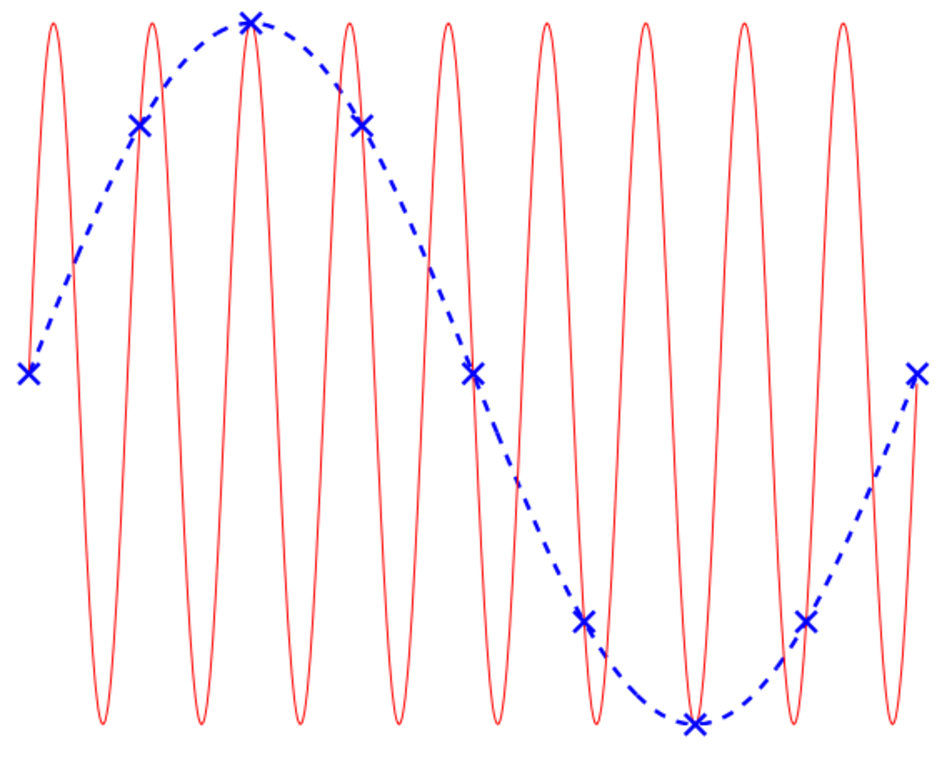
\includegraphics[width=0.8\textwidth]{alias}
  \caption{Aliaseffekten, signaler med frekvens över Nyquistfrekvensen går inte att skilja från signaler med lägre frekvens}
  \label{fig:alias}
\end{figure}
\FloatBarrier

\section*{Uppgift 11.2}
Betrakta 
\[\dot{y}(t) = u(t)\]
Ifall systemet ovan styrs av en dator är styrsignalen konstant under samplingsintervallet 
\[u(t) = u_k, \;\;\; kT \leq t \leq (k+1)T\]

\subsection*{a)}
Inför notationen $y_k = y(kt)$ och bestäm en relation mellan $y_{k+1},y_k$ och $u_k$
\qline
Låt $\mathcal{I}_k = [kT \leq t \leq (k+1)T]$ utgöra samplingsintervallen under samplingen och styrningen. Den datorberäknade insignalen $u(t)$ ges av konstant $u_k$ på varje $\mathcal{I}_k$. Den tidskontinuerliga utsignalen erhåller då förljande dynamik 
\[\dot{y}(t) = u_k, \;\;\; t \in \mathcal{I}_k\]
Denna differentialekvationen kan lätt lösas analytiskt genom att integrera 
\[\int_{kT}^{(k+1)T} \dot{y}(t) \de{t} = \int_{kT}^{(k+1)T}u_k \de{t}\] 
\[\Rightarrow y((k+1)T)-y(kT) = u_k T\]
Med den införda notationen ger detta att 
\[y_{k+1} - y_k = Tu_k\]
vilket är en differensevationen som beskriver systemet i diskret tid

\subsection*{b)}
Om P-reglering används, så att 
\[u_k = -Ky_k\]
och $y(0) = y_0$, för vilka $K$ blir det slutna systemet stabilt?
\qline
Slutna systemets differensekvation ges av
\begin{align*}
  y_{k+1} - y_k &= Tu_k = -TKy_k \\
  \Rightarrow y_{k+1} &= y_k - TKy_k = (1-TK)y_k
\end{align*}
Utsignalens uppförande när P-reglering används kan nu bestämmas rekursivt
\begin{align*}
  y_0 &= y_0 \\
  y_1 &= (1-TK)y_0 \\
  y_2 &= (1-TK)y_1 = (1-TK)^2 y_0 \\
  &\vdots \\
  y_m &= (1-TK)^m y_0
\end{align*}
Systemet är asymptotiskt stabilt då $|y^m| \to 0$ då $m \to \infty$, vilket sker precis då 
\[|1-TK| < 1 \Leftrightarrow -1 < 1-TK < 1 \Leftrightarrow 0 < K < \frac{2}{T}\]
Det slutna systemet är alltså stabilt ifall 
\[0 < K < \frac{2}{T}\]

\section*{Uppgift 11.1}
Använd Tustins formel på 
\[U(s) = KN 
\left(
  \frac{s+b}{s+bN}
\right)E(s)\]
vilket ger 
\[u(t) = \beta_1 u(t-T) + \alpha_1 e(t) + \alpha_2 e(t-T)\]
Vilka värden har $\alpha_1, \alpha_2$ och $\beta_1$ ifall 
\[T = 0.1, N = 10, b = 0.1, K = 2?\]
\qline
Tustins formel: 
\[p \approx \frac{2}{T} \frac{1 - q_T^{-1}}{1 + q_T^{-1}}\]
''$s$'' motsvarar derivering i laplacedomänen. Det är möjligt att inverslaplacetransformera överföringsfunktionen ovan och sedan approximera derivatorna med Tustins formel. Samma svar erhålls genom att formell byta ut symbolen ''$s$'' mot symbolen ''$p$'', så att
\begin{align*}
  F(s) &= F(p) \\
  &= KN 
    \left(
    \frac{p+b}{p+bN}
    \right) \\
  &= KN 
    \left(
    \frac{\frac{2}{T} \frac{1-q_T^{-1}}{1+q_T^{-1}}+b}{\frac{2}{T} \frac{1-q_T^{-1}}{1+q_T^{-1}}+bN}
    \right) \\
  &= KN 
    \left(
    \frac{bT(1+q_T^{-1}) + 2(1-q_T^{-1})}{bNT(1+q_T^{-1}) + 2(1-q_T^{-1})}
    \right) \\
  &= KN 
    \left(
    \frac{bT+2 + (bT-2)q_T^{-1}}{bNT+2+(bNT-2)q_T^{-1}}
    \right)
\end{align*}
Nu gäller att $u(T) = F(p)e(t)$ så att 
\[u(t) = KN 
    \left(
    \frac{bT+2 + (bT-2)q_T^{-1}}{bNT+2+(bNT-2)q_T^{-1}}
    \right)\]
vilket ger 
\[u(t) = -\frac{bNT-2}{bNT+2}u(t-T) + KN \frac{bT+2}{bNT+2}e(t) + KN \frac{bT-2}{bNT+2}e(t-T)\]
så att
\begin{align*}
  \beta_1 &= -\frac{bNT-2}{bNT+2} \approx 0.905 \\
  \alpha_1 &= KN \frac{bT+2}{bNT+2} \approx 19.14 \\
  \alpha_2 &= KN \frac{bT-2}{bNT+2} \approx -18.95
\end{align*}

\section*{Uppgift 11.3}
En insignal $u(t)$ mäts genom sampling efter att först passera genom ett förfilter enligt Figur \ref{fig:filtersamp}. 

\begin{figure}[h!]
  \centering
  \begin{tikzpicture}
    \node[block, text width=2cm] (samp) {Sampling};
    \node[block, left of=samp, node distance=3cm] (filt) {$\dfrac{1}{1+sT_1}$};
    \draw[wire] ++(-5,0) -- node[pos=0.5, above] {$u(t)$} (filt);
    \draw[wire] (filt) -- node[pos=0.5, above] {$\bar{y}(t)$} (samp);
    \draw[wire] (samp) -- node[pos=0.5, above] {$y_k$} ++(2,0);
  \end{tikzpicture}
  \caption{Sampling med förfilter av signalen $u(t)$}
  \label{fig:filtersamp}
\end{figure}
\FloatBarrier
Samplingen sker med period $T$. Insignalen ges av 
\[u(t) = u_0(t) + u_1(t)\]
där $u_0(t)$ är ''intressant'' och lågfrekvent, med frekvens inom 
\[0 < \omega < \frac{\pi}{T}\]
och 
\[u_1(t) = \sin{\omega_2 t}\]
är ett högfrekvent brus med 
\[\frac{\pi}{T} < \omega_2 < \frac{2\pi}{T}\]
Samplingen kommer således ge upphov till Aliaseffekten, så att 
\[y_k = y_k^{0} + y_k^{1}\]
där $y_k^{0}$ är ''intressant'' och $y_k^{1}$ utgör en störning som ej går att skilja från $y_k^{0}$. Aliaseffekten kan beskrivas matematiskt som att 
\[y_k^{1} = A \sin{(\omega_1 kT + \varphi)}\]
där 
\[0 < \omega_1 < \frac{\pi}{T}\]
så att $u_0(t)$ ej kan urskiljas.

\subsection*{a)}
Bestäm $A, \omega_1$ och $\varphi$.
\qline
Filtret 
\[G(s) = \frac{1}{1+sT_1}\]
är LTI (linjärt tids-invariant), så 
\[\bar{y}(t) = \bar{y}_0(t) + \bar{y}_t(t)\]
(där $\bar{Y}_0(s) = G(s)U_0(s)$ och $\bar{Y}_1(s) = G(s)U_1(s)$) \\
Efter att alla transienter dött ut gäller 
\[\bar{y}_1(t) = \bar{A}\sin{(\omega_2 t + \bar{\phi})}\]
där 
\begin{align*}
  \bar{A} &= |G(i\omega_2)| = \frac{1}{\sqrt{1+\omega_2^2T_1^2}} \\
  \bar{\phi} &= \arg{G(i\omega_2} = -\arctan{\omega_2 T}
\end{align*}
På grund av Aliaseffekten syns inte frekvenser över $\omega_N = \dfrac{\pi}{T}$ eftersom det går att addera $\dfrac{2\pi}{T}$ utan att förändra signalen. Hur kommer $\bar{y}_1(t)$ synas efter samplingen?
\begin{align}
  y_k^{1} &= \bar{y}_1(kT) \\
          &= \bar{A} \sin{(\omega_2 kT + \bar{\phi})} \\
          &= \bar{A} \sin{(\pi - \omega_2 kT - \bar{\phi})} \\
          &= \bar{A} \sin{(2\pi k + \pi - \omega_2 kT - \bar{\phi})} \\
          &= \bar{A} \sin{\left( \left(\frac{2\pi}{T}-\omega_2\right)kT + \pi - \bar{\phi}\right)}
\end{align}
där 
\[\frac{2\pi}{T} - \omega_2 < \frac{\pi}{T}\]
eftersom 
\[\frac{\pi}{T} < \omega_2 < \frac{2\pi}{T}\]
denna frekvens kommer vara synlig efter samplingen! Alltså erhålls
\begin{align*}
  \omega_1 &= \frac{2\pi}{T} - \omega_2 \\
  A &= \bar{A} = \frac{1}{\sqrt{1+\omega_2^2 T_1^2}} \\
  \varphi &= \pi - \bar{\phi} = \pi + \arctan{\omega_2 T_1}
\end{align*}

\subsection*{b)}
Förfiltret kan användas för att dämpa bort störsignalen. Vilken är den lägsta amplitud som kan uppnås ifall $u_0$:s amplitud inte ska dämpas mer än $\sqrt{2}$.
\qline
Förfiltret dämpar signaler med
\[\frac{1}{\sqrt{1+\omega_2^2 T_1^2}}\]
målet är att dämpa signaler med frekvens inom
\[\frac{\pi}{T} < \omega < \frac{2\pi}{T}\]
så mycket som möjligt, men signaler med frekvenser inom 
\[0 < \omega < \frac{\pi}{T}\]
bör inte dämpas med mer än 
\[\frac{1}{\sqrt{2}}\]
Detta kan uppnås genom att variera $T_1$ så att förfiltrets bandbredd ges av 
\[\frac{\pi}{T}\]
Bestäm först förfiltrets bandbredd 
\begin{align*}
  \frac{1}{\sqrt{1+\omega_B^2 T_1^2}} &= \frac{1}{\sqrt{2}}  \\
  \Leftrightarrow 1+\omega_B^2 T_1^2 &= 2 \\
  \Leftrightarrow \omega_B &= \frac{1}{T_1}
\end{align*}
Välj nu $T_1$ så att
\begin{align*}
  \frac{1}{T_1} &= \frac{\pi}{T} \\
  \Rightarrow T_1 &= \frac{T}{\pi}
\end{align*}
Med detta $T_1$ kommer signaler med frekvens lägre än $\dfrac{\pi}{T}$ dämpas mer än $\sqrt{2}$, och signaler med högre frekvens dämpas mindre än $\sqrt{2}$. Specifikt gäller att störsignalen dämpas med 
\[\frac{1}{\sqrt{1+\omega_2^2 \frac{T^2}{\pi^2}}}\]


\end{document}

